% \setchapterpreamble[u]{\margintoc}
\chapter{Introduction et résumé en français}
\labch{french}

\warn{
  This chapter is the French translation of \nrefch{intro}.
  You can also skip to the \hyperlink{toc}{table of contents}.
}

\selectlanguage{french}

La théorie des types se trouve à l'interface entre programmation et logique
formelle, les deux mondes se nourissant l'un l'autre. Des assistants de preuve
peuvent être basés dessus, ce qui en fait également des langages de
programmation à part entière, avec l'avantage supplémentaire de produire des
programmes certifiés.

Mon intérêt principal réside dans l'étude de la théorie des types tout en s'appuyant sur les outils qu'elle fournit :

My main interest lies in the study of type theory while relying on the tools it
provides: j'étudie la théorie des types \emph{au sein même} de la théorie des
types.
Ainsi, je me suis concentré sur la formalisation de la théorie des types dans
l'assistant de preuve \Coq~\sidecite[-0.7cm]{coq} et particuliètement sur
deux points:
\marginnote[0.7cm]{
  La \emph{reflection} et la notion d'égalité faible sont définies en
  \arefsubsecfr{ett-def} et \arefsubsecfr{wtt} respectivement, les deux dans
  le \refch{flavours}.
}
\begin{itemize}
  \item Comment peut-on transformer efficacement une preuve utilisant une notion
  très forte d'égalité appelée \emph{reflection}, en une preuve s'appuyant sur
  une notion très faible d'égalité ?
  \item Comment peut-on accroître la confiance dans notre système, dans mon
  cas \Coq, en utilisant ce système lui-même comme cadre pour l'étudier ?
\end{itemize}

\paradot{Contributions}
Mes contributions se trouvent principalement dans \avrefpartfr{elim-reflection}
et \avrefpartfr{coq-in-coq}, correspondant aux publications
suivantes~\sidecite{winterhalter:hal-01849166,sozeau2019coq,sozeau:hal-02167423}.
Bien que les chapitres précédant ces deux parties soient principalement
introductifs et correspondent à un état de l'art approximatif, ils contiennent
en réalité d'autres contributions, à savoir le travail que j'ai fait avec Andrej
Bauer sur le modèle cardinal dans \nrefch{models} actuellement non publié, et le travail avec Andrej Bauer et Philipp Haselwarter sur la formalisation de la
théorie des types appelée \ftt~\sidecite[-0.1cm]{formaltypetheory} et que je
présente brièvement dans \nrefch{formalisation}.

\section{Assistans à la preuve\sidenote{On dit souvent ``assistant de preuve'', et je vais également le faire, mais il semblerait que la formulation ``assistant à la preuve'' soit plus correcte.}}

L'un de mes objectifs est d'améliorer et de mieux comprendre les assistants de
preuve, mais qu'est-ce qu'un assistant de preuve?
Je pense que nous pouvons les voir comme des chatbots --- c'est-à-dire des
programmes avec lesquels vous pouvez converser --- qui sont là pour vous aider à
énoncer et à prouver des théorèmes.
Ils ne sont pas particulièrement intelligents et ne feront pas le travail pour
vous, mais ils sont très ennuyeux car ils ne comprennent pas toujours ce que
vous dites et vous devez être très précis ou ils vous feront remarquer vos
erreurs.

\marginnote[1.2cm]{
  L'utilisateur aura des bulles bleues, légèrement à gauche, tandis que
  l'assistant de preuve répondra en vert (réponse positive) ou en rouge
  (réponse négative) sur le côté droit.
}%
\begin{center}
  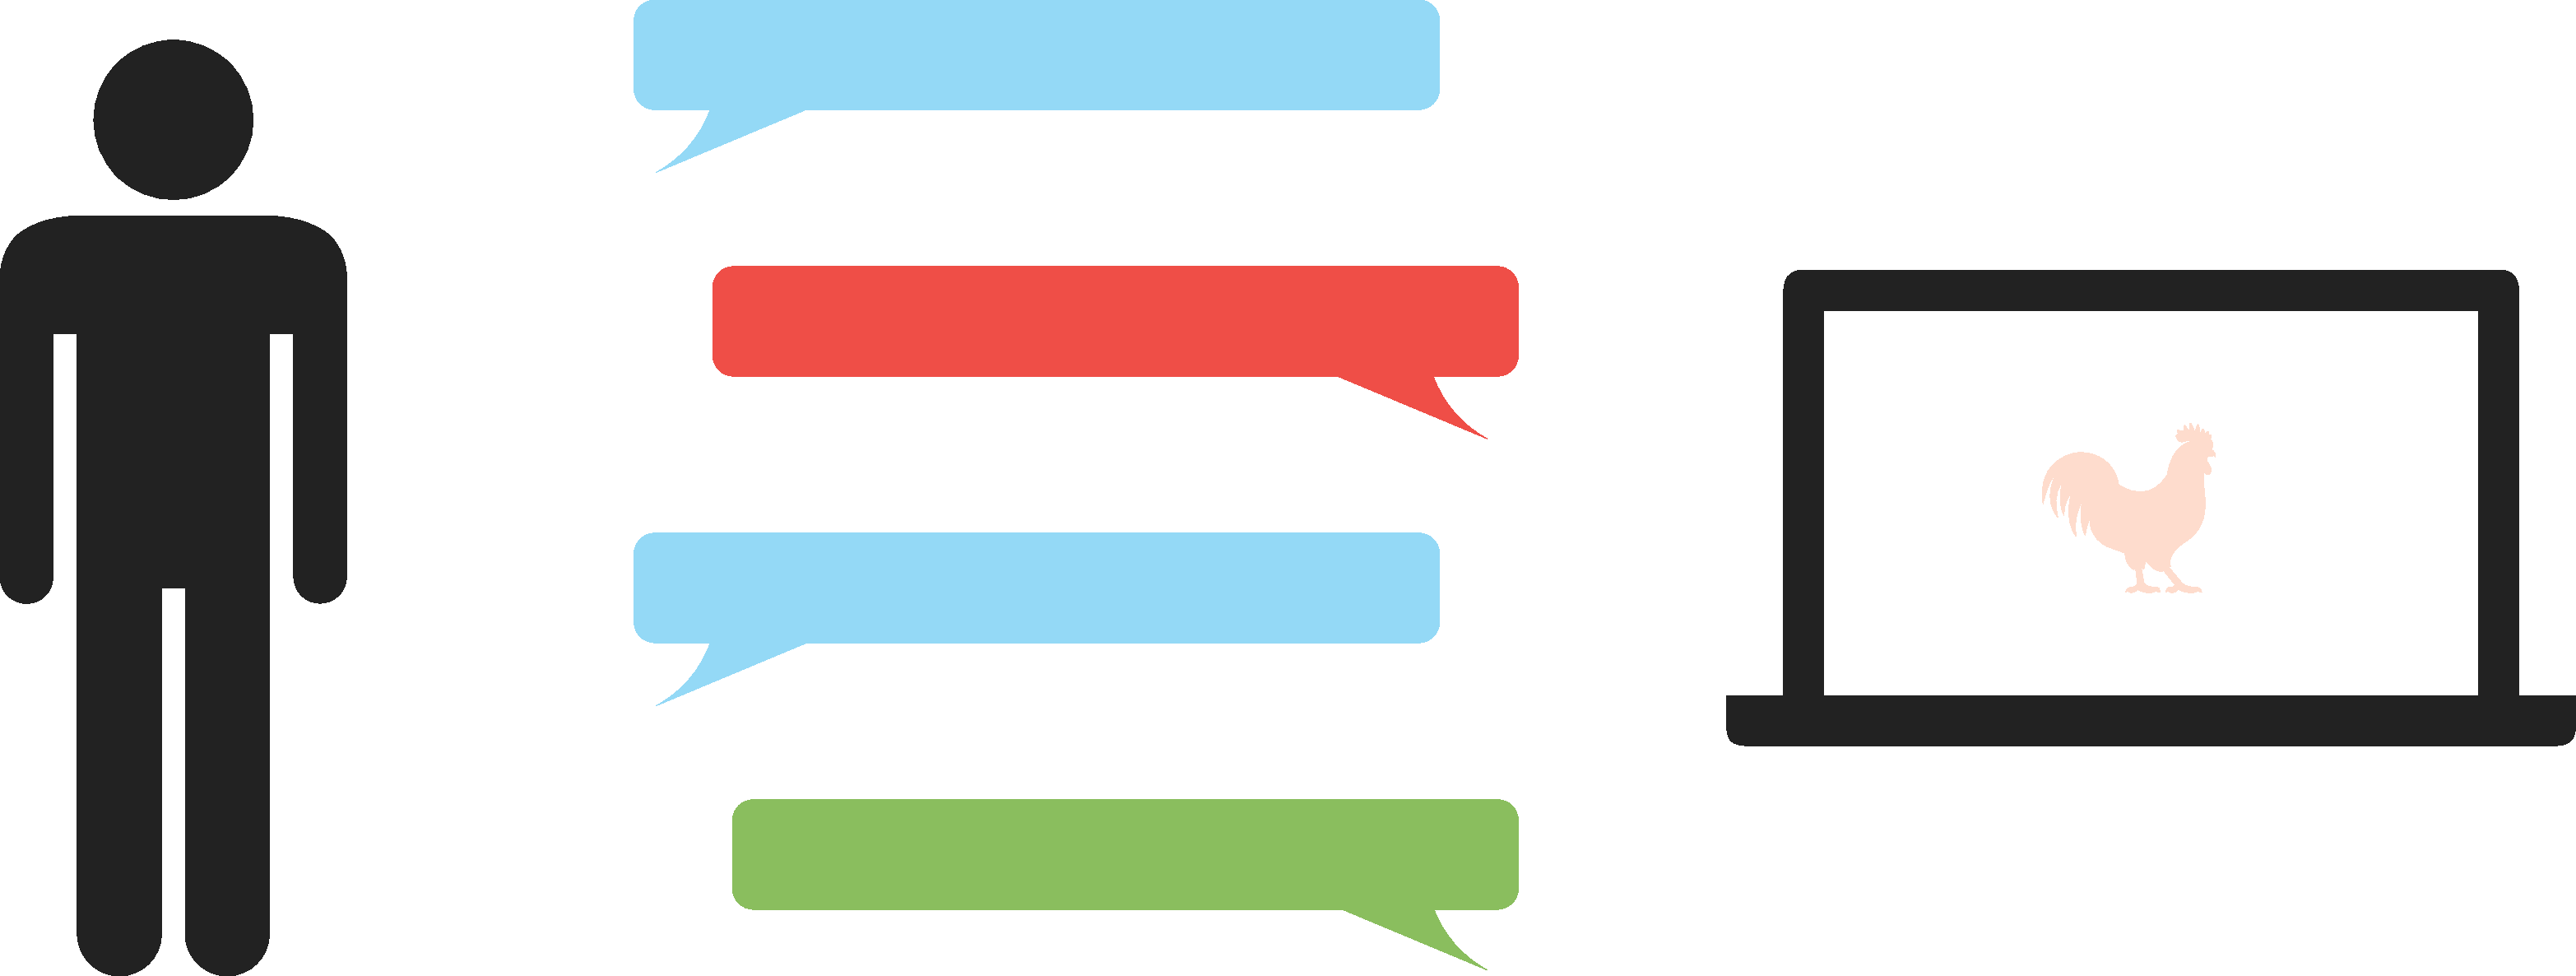
\includegraphics[width=0.6\textwidth]{coq-chatbot.pdf}
\end{center}

Ici, je représente l'utilisateur à gauche, en conversation avec l'assistant
de preuve, à droite, que j'imagine comme un ordinateur portable avec un coq à
l'intérieur.

Voyons maintenant en détail comment une telle conversation peut se dérouler.

\begin{center}
  
\includegraphics[width=0.8\textwidth]{modern-art.pdf}
\end{center}

\marginnote[0.1cm]{
  Quand je dis qu'ils sont d'accord, je veux dire que, en particulier,
  l'assistant de preuve a des connaissances de base sur les chats et les boîtes,
  par exemple, vous n'avez pas besoin de montrer qu'un chat est un félin.
  Il sait également ce que contient chaque boîte, par exemple que la quatrième
  boîte contient un chat rouge.
}
Cette œuvre d'art moderne sera le cadre de l'échange entre l'utilisateur et
l'assistant de preuve, et nous supposerons qu'ils sont tous les deux d'accord
sur ce cadre.
Nous avons des chats dans des boîtes (bien que l'un des chats soit plutôt un
lion), de différentes couleurs et soumis à différentes forces de gravitation.

Au début, l'utilisateur fait connaître son but à l'assistant de preuve, en
disant pour quel théorème il a besoin de son aide.

\begin{center}
  
\includegraphics[width=0.8\textwidth]{iwanterror-fr.pdf}
\end{center}

La phrase ci-dessus ne ressemble pas à un énoncé que nous pouvons prouver, et
l'assistant de preuve se plaindra à juste titre.

\begin{center}
  
\includegraphics[width=0.8\textwidth]{error-incomplete-fr.pdf}
\end{center}

En effet, nous sommes allé trop vite et avons oublié la moitié de ce que nous voulions dire. Cette fois, on lui donne une phrase complète.

\begin{center}
  
\includegraphics[width=0.8\textwidth]{iwant-is-fr.pdf}
\end{center}

Maintenant, l'énoncé est légèrement incorrect, ou pas assez précis pour notre
gentil assistant.

\begin{center}
  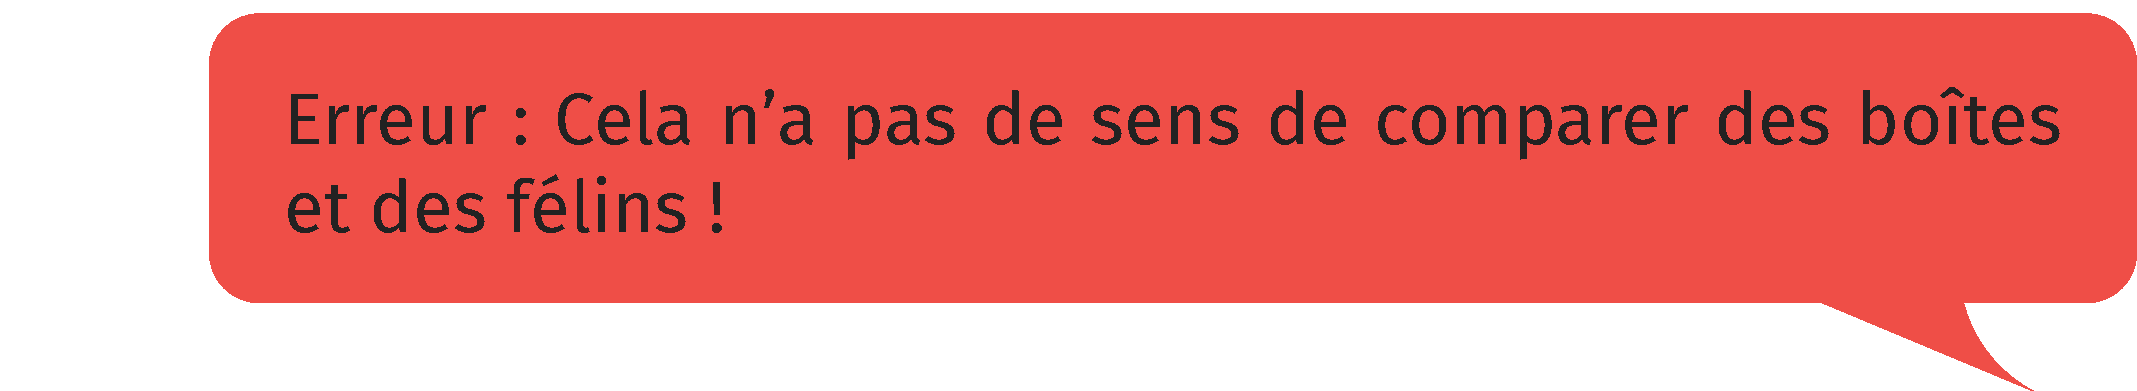
\includegraphics[width=0.8\textwidth]{error-box-feline-fr.pdf}
\end{center}

Nous devons réviser le théorème voulu et réaliser que nous ne voulons pas
prouver que toutes les boîtes sont des félins, bien qu'un humain puisse
comprendre ce que nous entendons par là, mais que toutes les boîtes
contiennent, chacune, un félin.

\begin{center}
  
\includegraphics[width=0.8\textwidth]{box-contains-feline-fr.pdf}
  
\includegraphics[width=0.8\textwidth]{how-to-prove-fr.pdf}
\end{center}

L'assistant de preuve a maintenant compris ce que nous voulions dire. La partie
interactive de la preuve commence maintenant. Nous voulons prouver une propriété
sur les boîtes, comme il y en a quatre à considérer, nous pouvons dire à
l'assistant de preuve que nous avons l'intention d'examiner chaque cas, un par
un.

\begin{center}
  
\includegraphics[width=0.8\textwidth]{convo7-fr.pdf}
  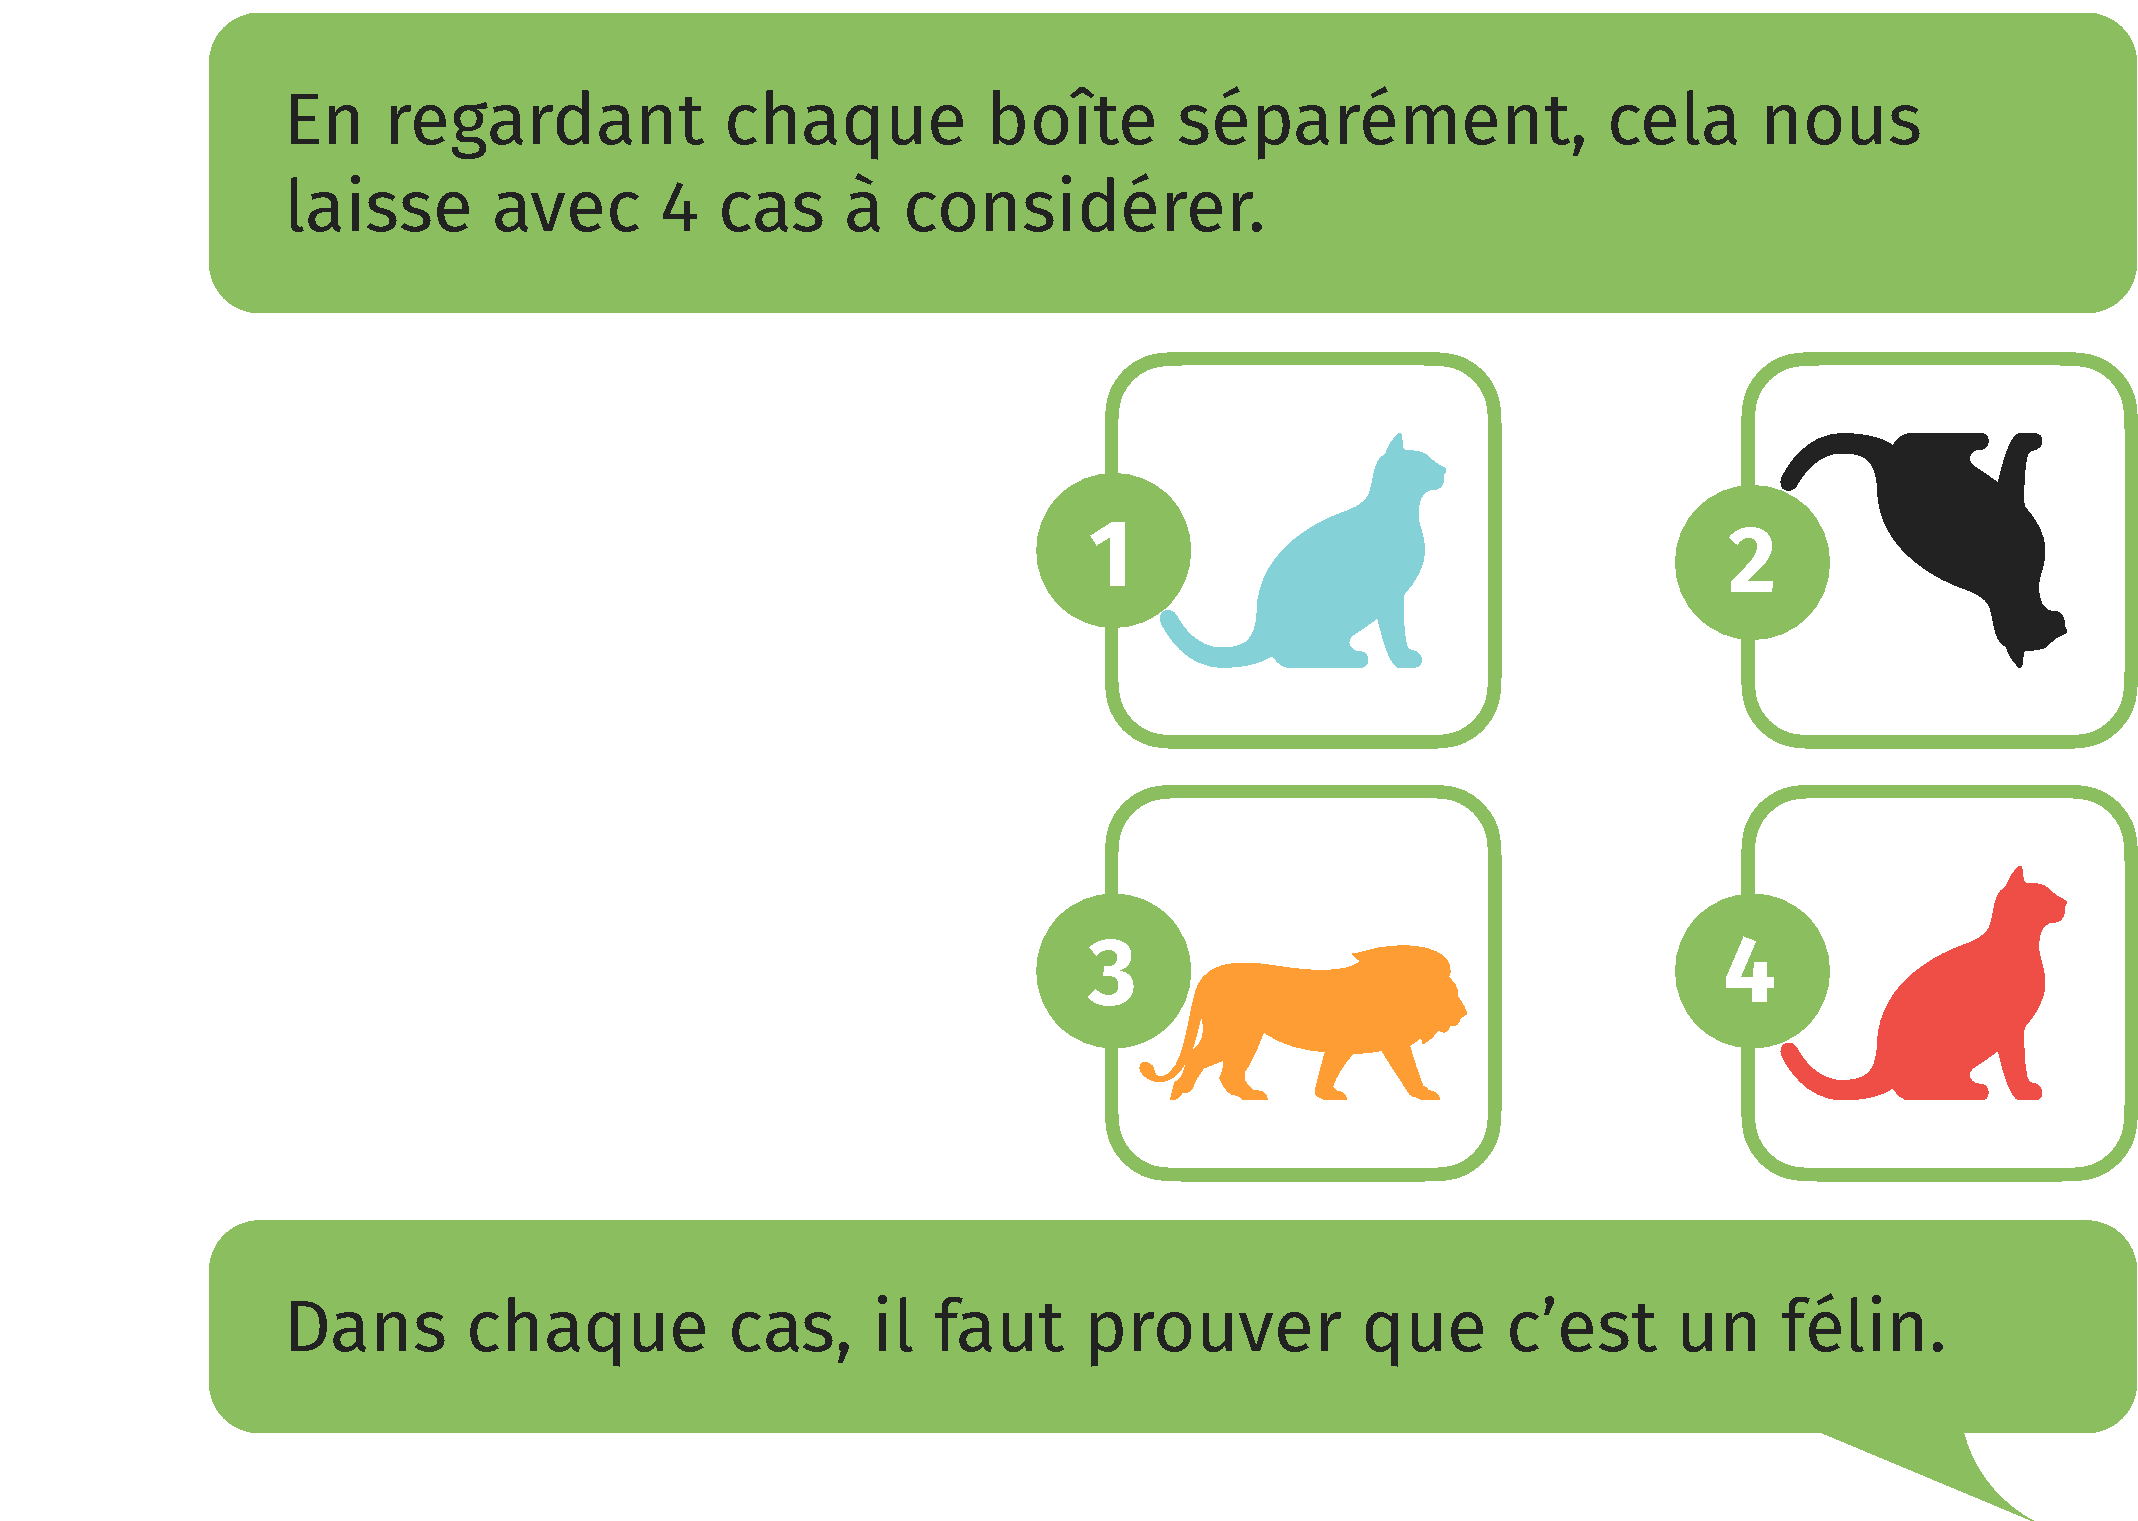
\includegraphics[width=0.8\textwidth]{convo8-fr.pdf}
\end{center}

On nous présente quatre cas, et autant d'énoncés à prouver.
Dans ce cas, nous sommes plutôt paresseux, d'autant plus que les quatre cas
seront similaires. Heureusement pour nous, l'assistant de preuve est capable de
comprendre que nous voulons traiter plusieurs cas de manière similaire,
\emph{et} est également capable de faire des preuves très basiques sans
l'intervention de l'utilisateur.

\begin{center}
  
\includegraphics[width=0.8\textwidth]{convo9-fr.pdf}
  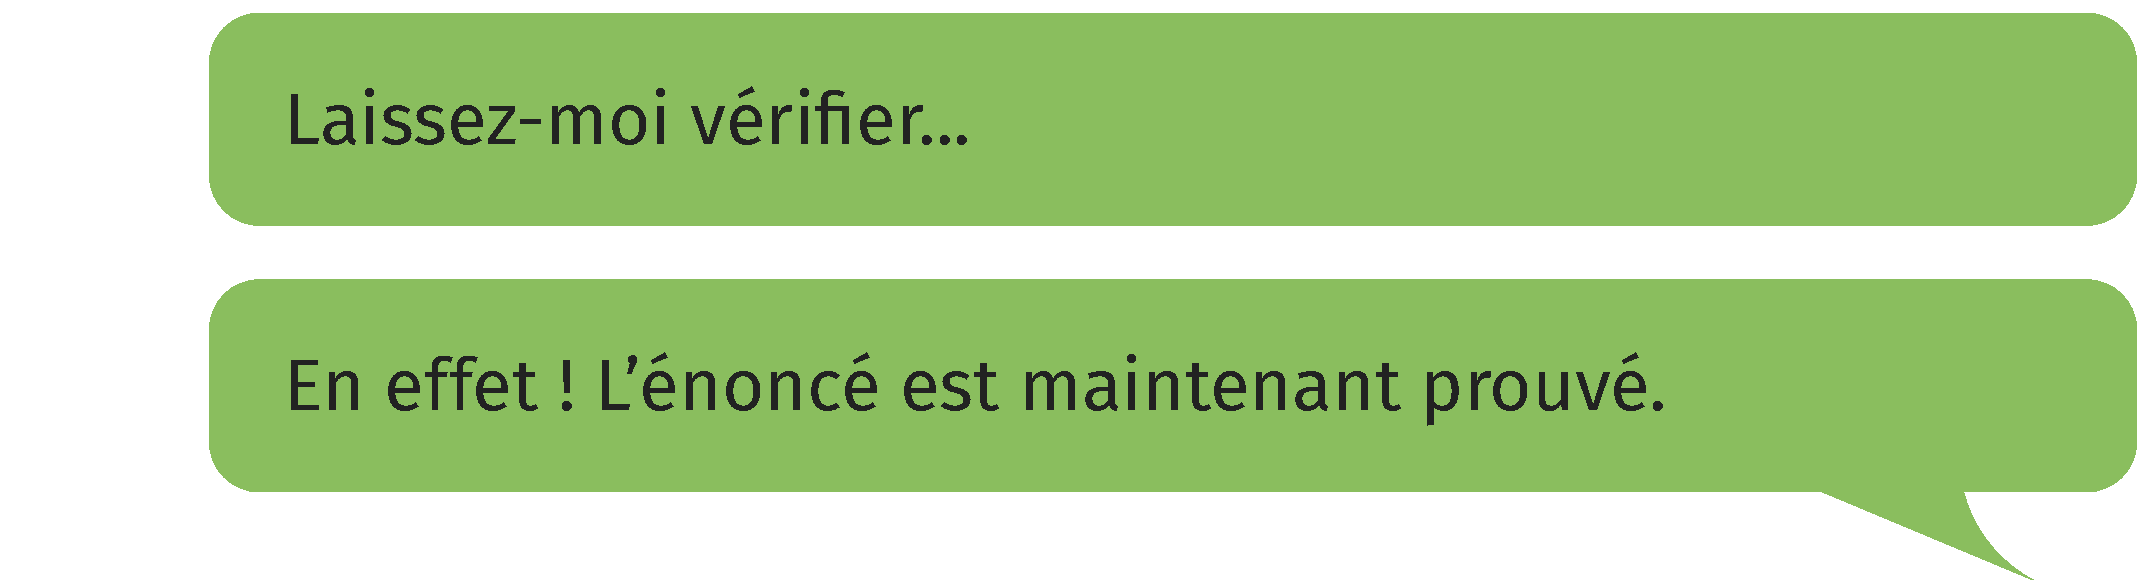
\includegraphics[width=0.8\textwidth]{convo10-fr.pdf}
\end{center}

Une fois la preuve terminée, l'assistant de preuve vous le dit et vous pouvez
passer à d'autres théorèmes pour le prouver. J'ai déjà montré que vous devez
être explicite et non ambigu lorsque vous parlez à l'assistant de preuve. Vous
devez également être correct.
L'assistant de preuve ne se fiera pas aveuglément à ce que vous dites.
%
Considérons maintenant un théorème qui n'est pas prouvable.

\begin{center}
  
\includegraphics[width=0.8\textwidth]{convo11-fr.pdf}
  
\includegraphics[width=0.8\textwidth]{how-to-prove-fr.pdf}
  
\includegraphics[width=0.8\textwidth]{convo7-fr.pdf}
  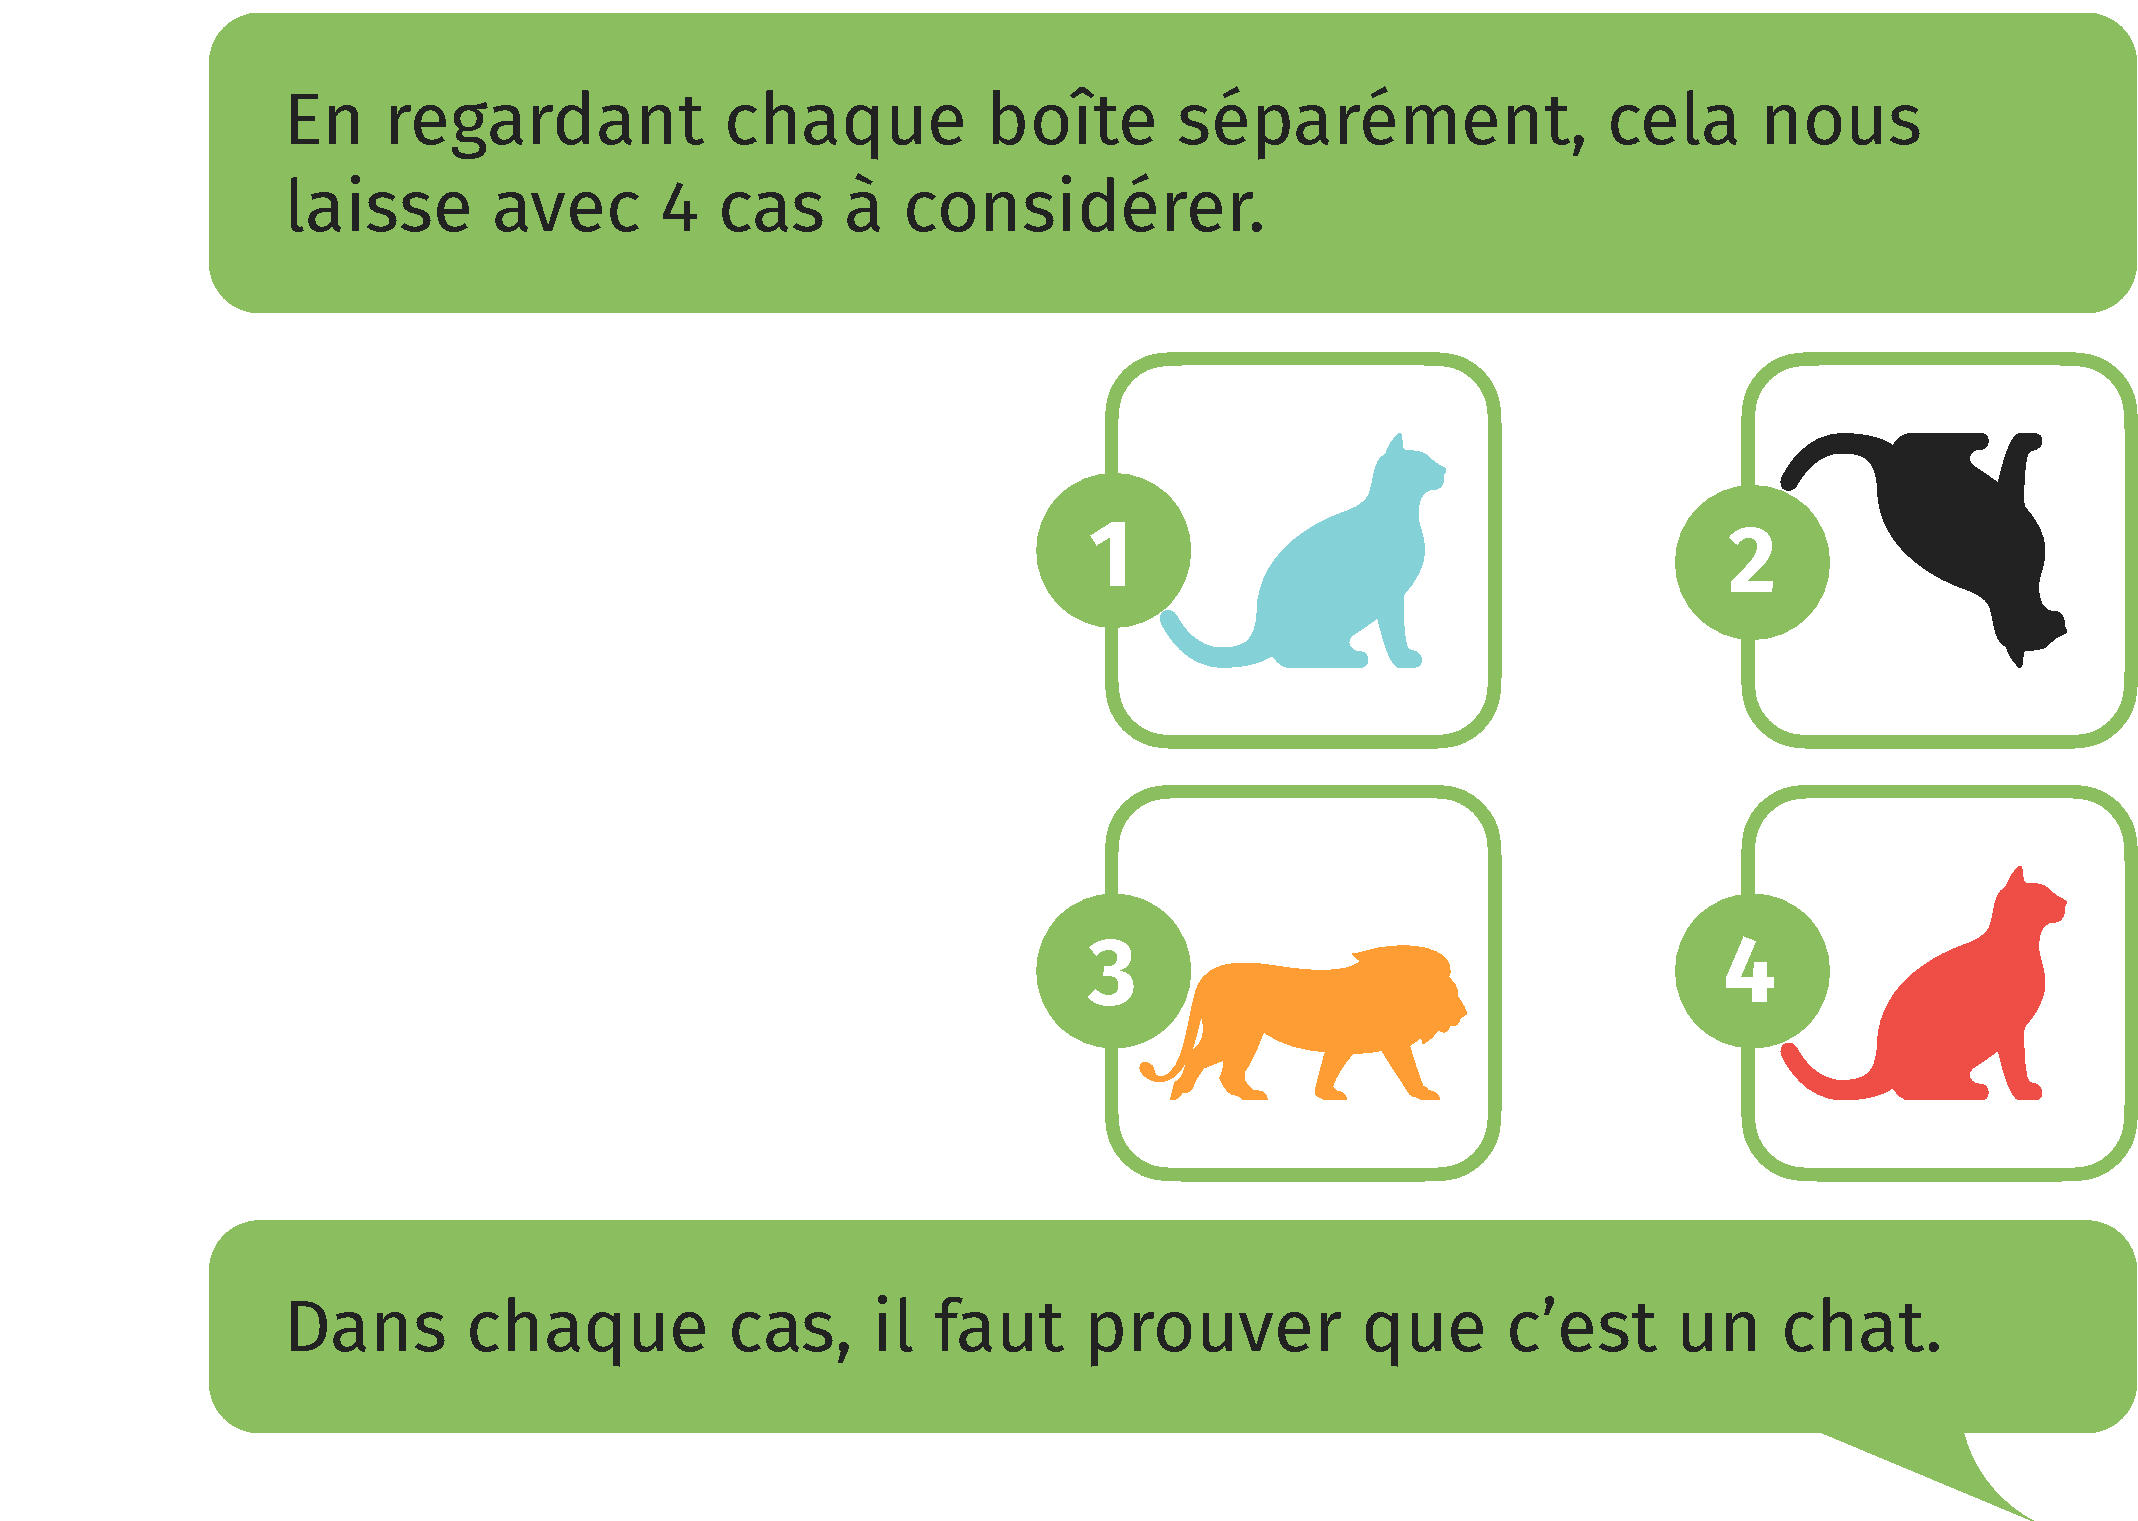
\includegraphics[width=0.8\textwidth]{convo12-fr.pdf}
  
\includegraphics[width=0.8\textwidth]{convo9-fr.pdf}
  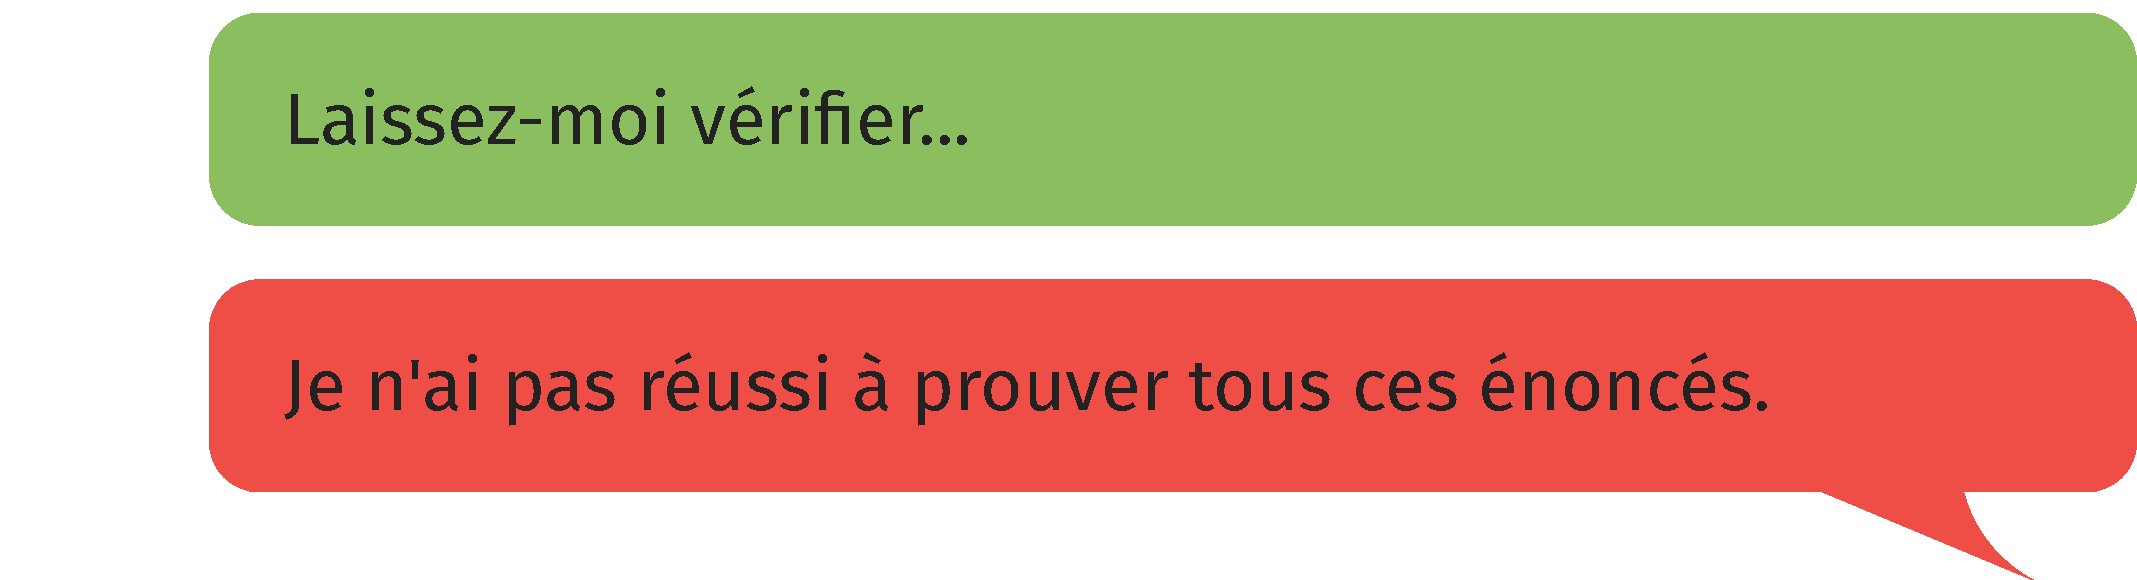
\includegraphics[width=0.8\textwidth]{convo13-fr.pdf}
\end{center}

Ici, l'assistant de preuve nous dit que tous les cas ne sont pas triviaux, nous
décidons donc de les examiner un par un pour comprendre ce qui ne va pas.

\begin{center}
  
\includegraphics[width=0.8\textwidth]{convo-focus-fr.pdf}
  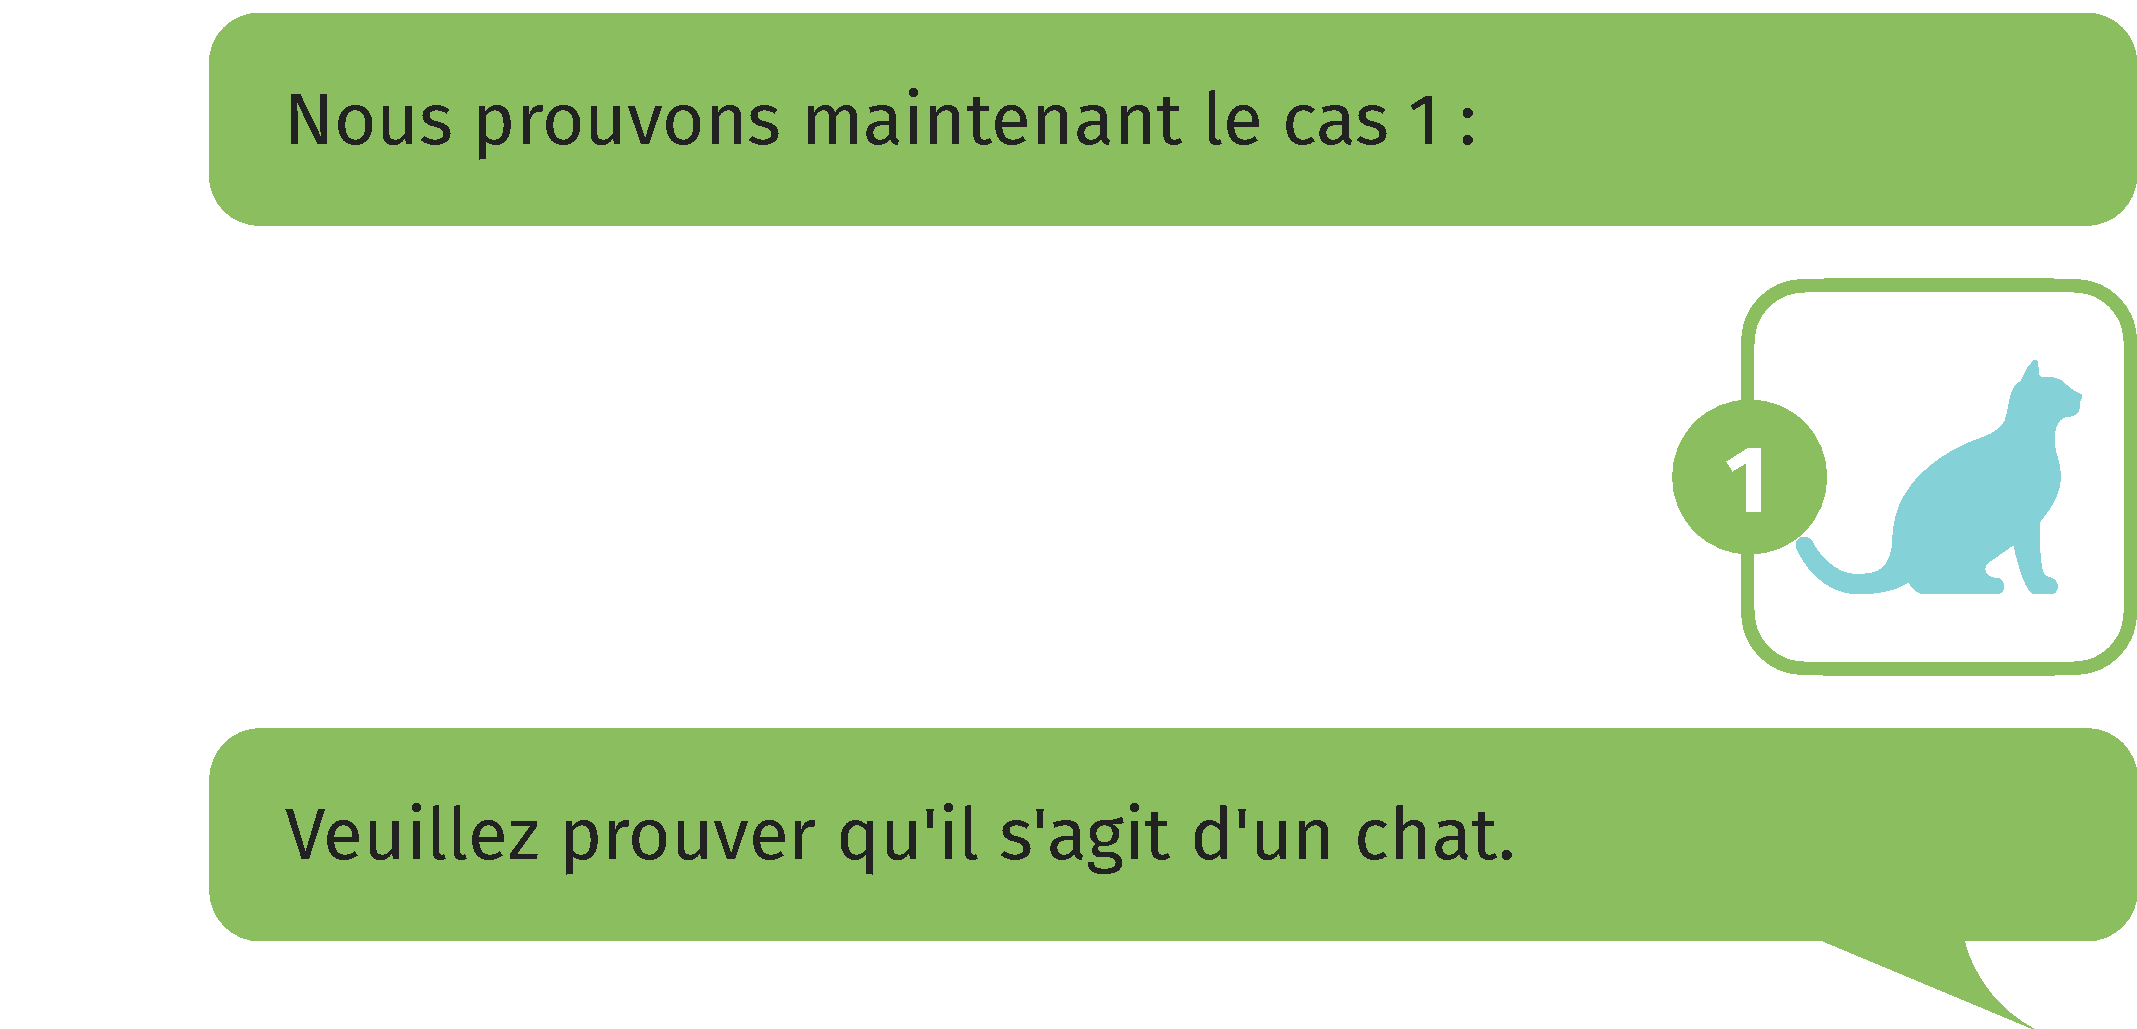
\includegraphics[width=0.8\textwidth]{convo-case1-fr.pdf}
\end{center}

Lorsque nous nous concentrons sur un cas, l'assistant de preuve nous rappelle ce
que nous devons prouver spécifiquement. Ici, nous revenons à l'utilisation de
notre stratégie antérieure et disons simplement que c'est évident.

\begin{center}
  
\includegraphics[width=0.8\textwidth]{convo-trivial-fr.pdf}
  
\includegraphics[width=0.8\textwidth]{convo-indeed-fr.pdf}
  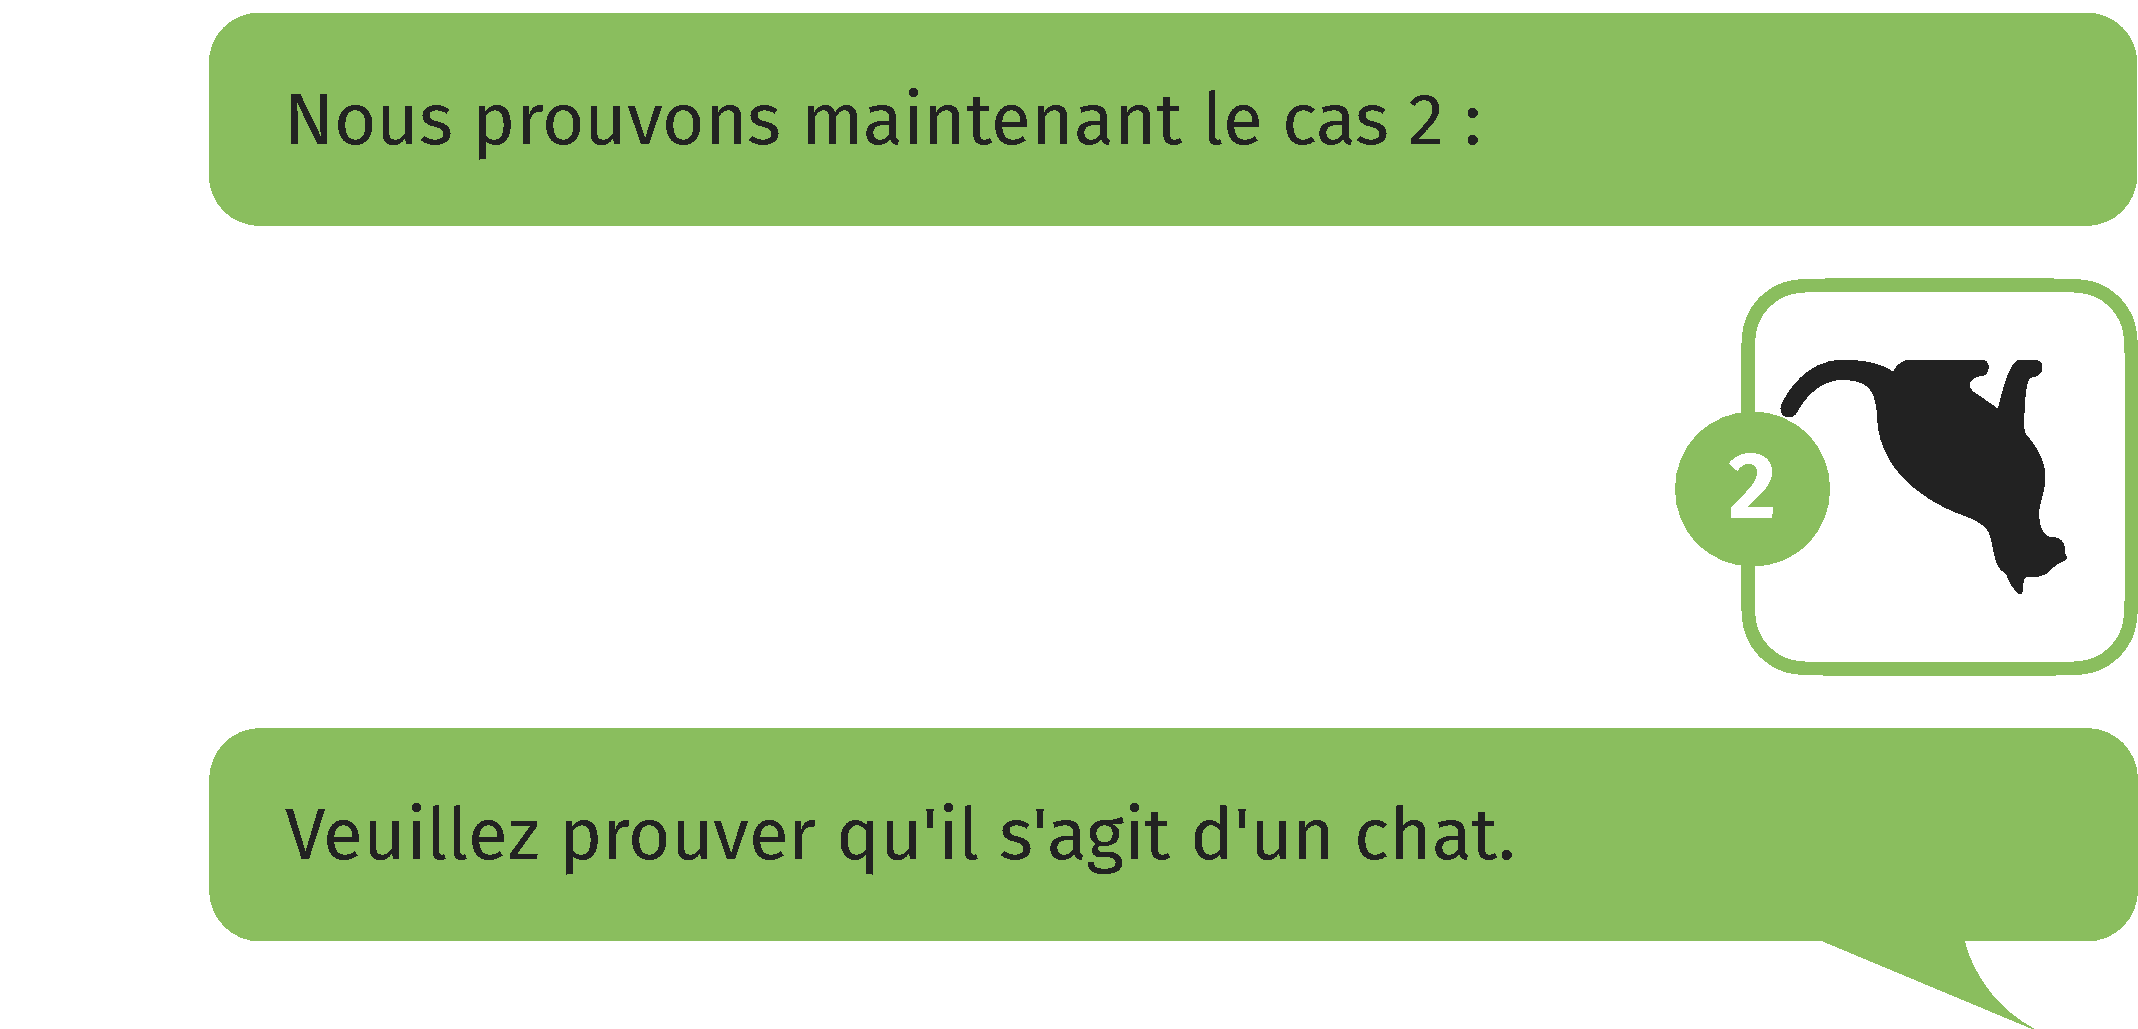
\includegraphics[width=0.8\textwidth]{convo-case2-fr.pdf}
  
\includegraphics[width=0.8\textwidth]{convo-trivial-fr.pdf}
  
\includegraphics[width=0.8\textwidth]{convo-indeed-fr.pdf}
  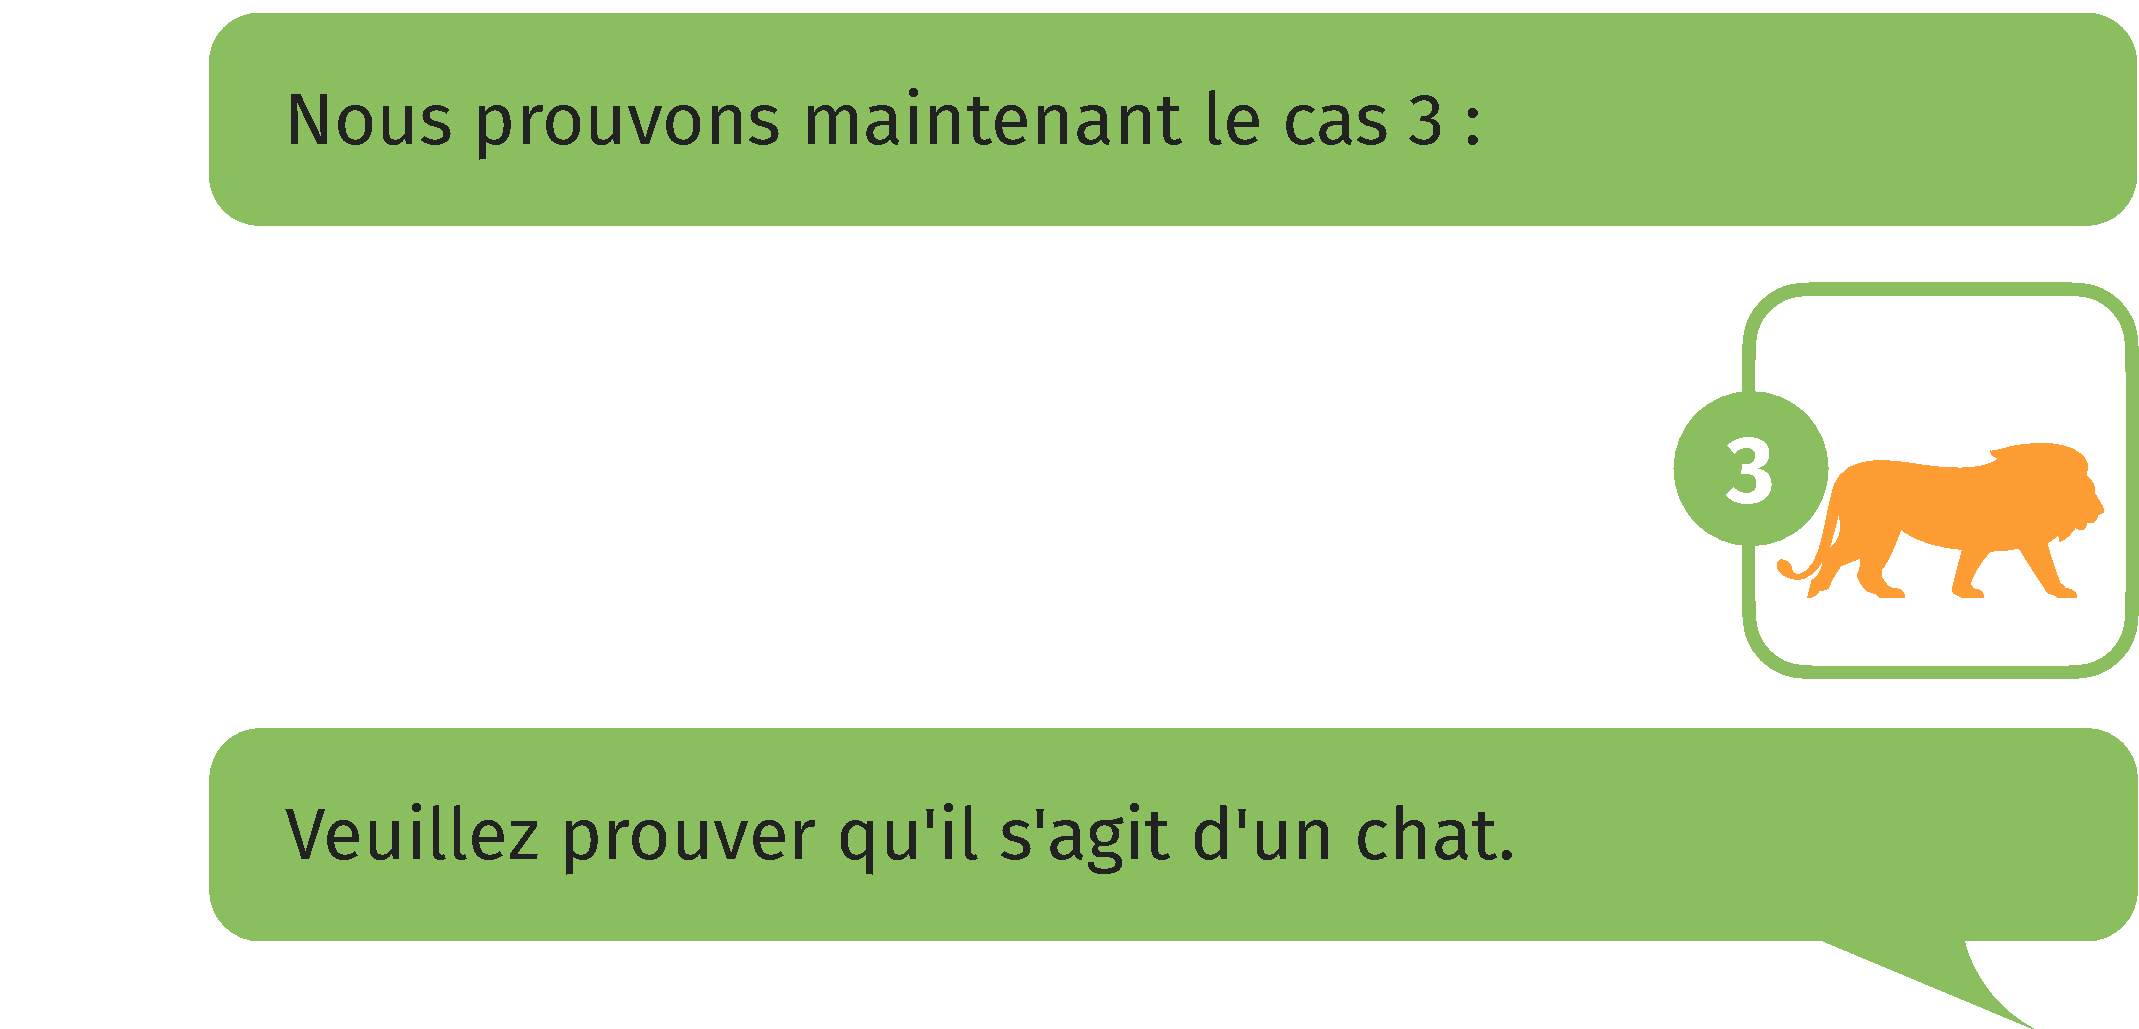
\includegraphics[width=0.8\textwidth]{convo-case3-fr.pdf}
  
\includegraphics[width=0.8\textwidth]{convo-abort-fr.pdf}
\end{center}

Cette fois, nous voyons que nous n'avons pas de chat donc nous n'essayons même
pas de le prouver.
Nous abandonnons la preuve, c'est-à-dire que nous renonçons à prouver un
énoncé que nous savons maintenant faux.
Une chose importante à noter ici est que l'assistant de preuve ne sait toujours
pas que l'énoncé est incorrect, mais seulement que la tentative de preuve était elle-même invalide.
Nous pouvons montrer que l'énoncé est faux en prouvant l'inverse :

\begin{center}
  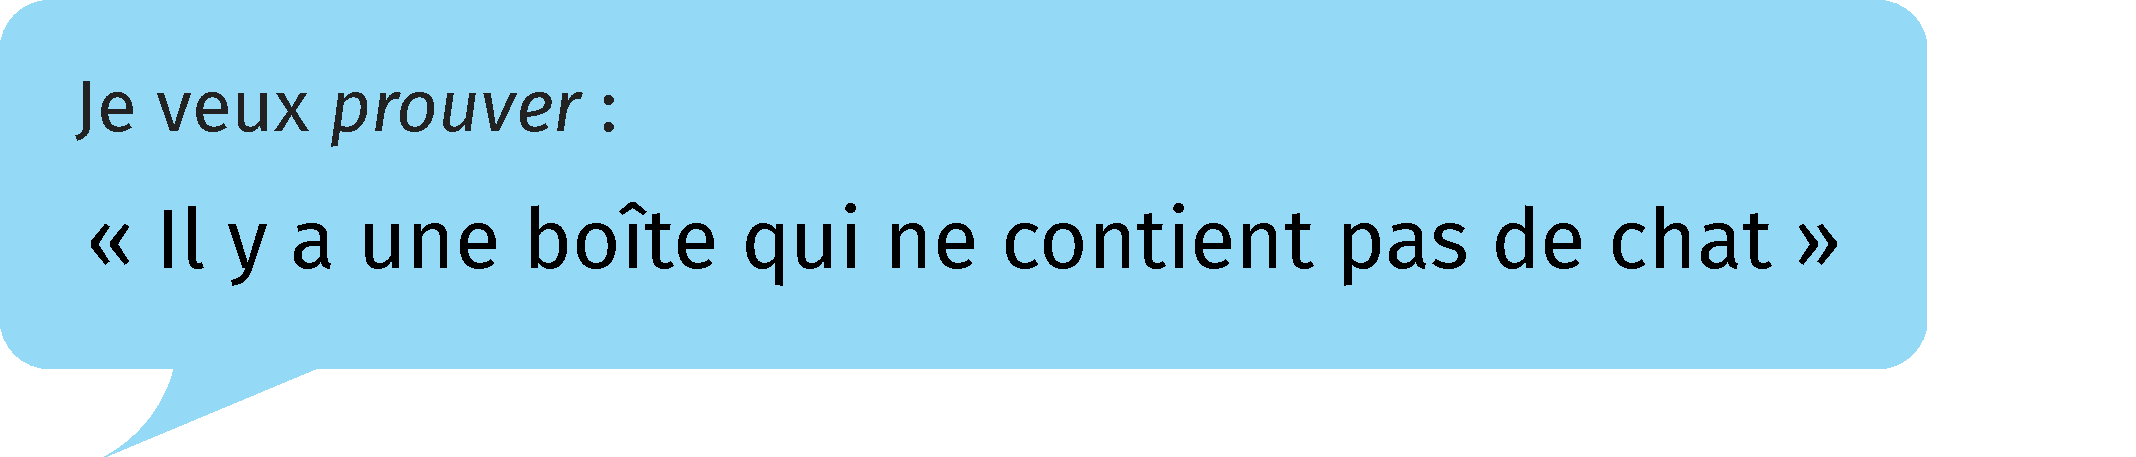
\includegraphics[width=0.8\textwidth]{conv-exists-fr.pdf}
  
\includegraphics[width=0.8\textwidth]{how-to-prove-fr.pdf}
\end{center}

La façon la plus simple de prouver que quelque chose existe est de fournir ce
que l'on appelle un \emph{témoin} d'existence. Ici, nous recherchons une boîte
qui ne contient pas de chat, il n'y a qu'une seule boîte sans chat, comme nous l'avons découvert lors de notre précédente épreuve, la troisième.

\begin{center}
  
\includegraphics[width=0.8\textwidth]{convo-take-third-fr.pdf}
  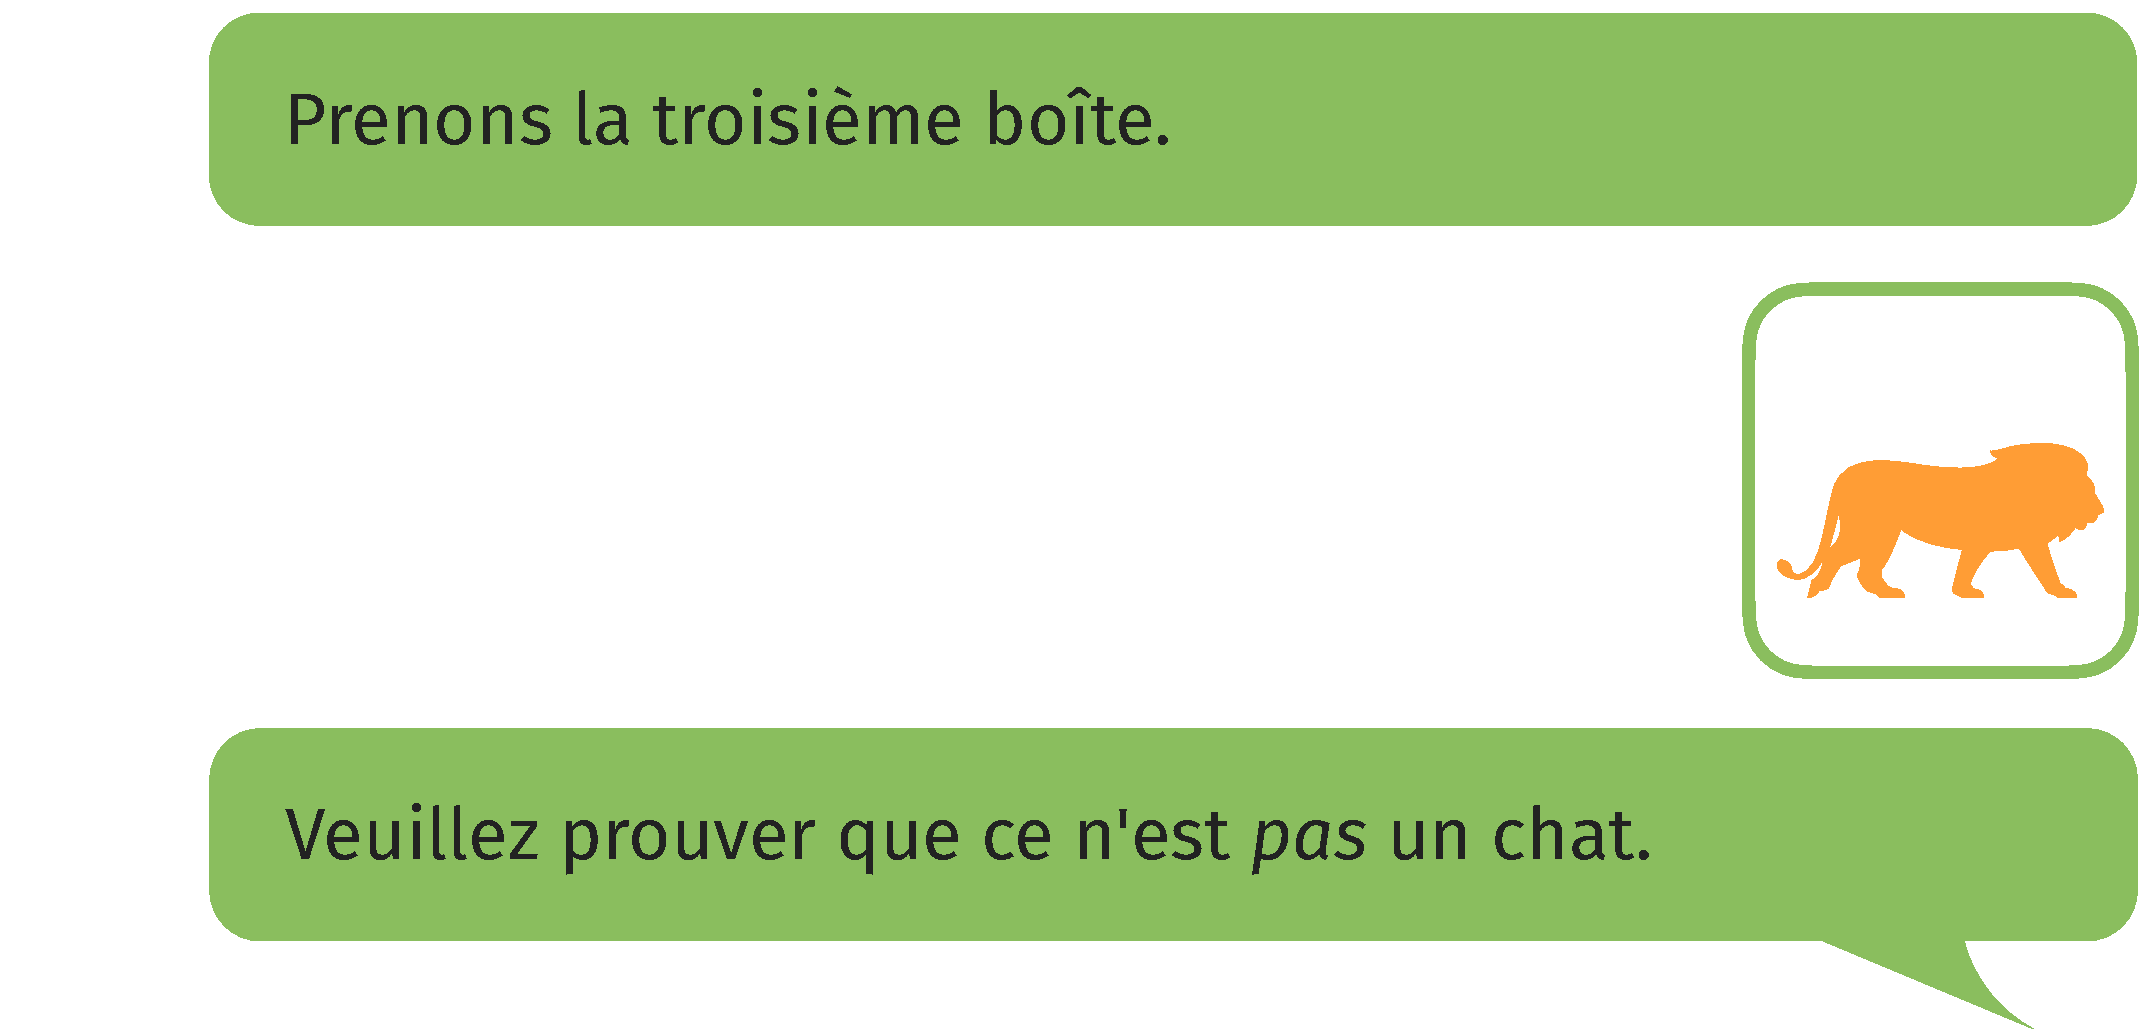
\includegraphics[width=0.8\textwidth]{convo-after-exists-fr.pdf}
  
\includegraphics[width=0.8\textwidth]{convo-trivial-fr.pdf}
  
\includegraphics[width=0.8\textwidth]{convo-indeed-fr.pdf}
  
\includegraphics[width=0.8\textwidth]{convo-proven-fr.pdf}
\end{center}

Un assistant de preuve nous aide donc à la fois à faire des preuves en
construisant des parties de la preuve lui-même et à vérifier qu'elles sont
correctes, par exemple en s'assurant qu'on n'a pas oublié un cas où nous avions
un lion plutôt qu'un chat.

Les assistants d'épreuve sont également intéressants et utiles pour d'autres
personnes que l'utilisateur qui fait la preuve. Disons que j'ai prouvé un
théorème compliqué en utilisant mon assistant de preuve préféré, les personnes
qui font confiance à mon assistant de preuve devront simplement lui demander
s'il est d'accord avec mon affirmation.
En fait, les assistants de preuve génèrent généralement ce que l'on appelle des
\emph{certificats} qui peuvent être vérifiés par d'autres sans avoir à
comprendre les détails de la preuve.

\begin{center}
  
\includegraphics[width=0.5\textwidth]{cerificate-fr.pdf}
\end{center}
\marginnote[-3cm]{
  L'image peut être trompeuse, je parle vraiment d'un objet concret que les gens
  peuvent analyser à l'aide de leur propre assistant de preuve pour vérifier
  qu'une preuve est bien valide.
}

Quand bien même, pourquoi devrions-nous faire confiance à l'assistant de
preuve ? Que pouvons-nous prouver exactement avec des assistant à la preuve ?
Et comment pouvons-nous les améliorer ?
Une partie de mon travail est centrée sur ces questions, et sur l'étude des
assistants de preuve basés sur ce que l'on appelle la théorie des types.

\section{Preuves, types et programmes}

Afin d'expliquer le titre ``Formalisation et méta-théorie de la théorie des
types'', j'ai besoin d'expliquer ce qu'est la \emph{théorie des types}.
Avant cela, je pense que je dois introduire la \emph{théorie de la preuve}
(\refch{proof-theory}) : l'étude des preuves elles-mêmes.
En effet, pour construire un assistant de preuve, il faut comprendre ce qu'est
une preuve, formellement, c'est-à-dire en termes très précis et non ambigus.

Il s'avère que certaines notions formelles de preuves ont des relations complexes avec la programmation comme nous le verrons dans le \refch{simple-types}.
L'idée est que les programmes peuvent être considérés comme des preuves et les
preuves comme des programmes.
Par exemple, la preuve qu'un proposition \(A\) implique la proposition \(B\)
est un programme qui prend une preuve de \(A\) en entrée et renvoie une preuve
de \(B\) en sortie.
Un tel programme est de type \(A \to B\). Les types sont un moyen de décrire les
données renvoyées par un programme. Les étudiants sont souvent amenés à écrire
la fameuse fonction de test d'une année bissextile qui, étant donnée une année
sous forme d'entier (décrit par le type \mintinline{ocaml}{int}), répond s'il
s'agit d'une année bissextile ou non. Cette information binaire --- oui ou non
--- est encodée dans ce que nous appelons des booléens
(\mintinline{ocaml}{bool}).
La correspondance de Curry-Howard indique que les programmes de type \(A\)
peuvent être considérés comme des preuves de la proposition \(A\) et vice-versa.

Danse le \refch{dependent-types}, je décris enfin ce que j'appelle la théorie
des types.
La théorie des types est un cadre qui tire parti de cette correspondance et est donc au cœur d'assistants de preuve bien connus tels que
\Coq~\sidecite[-1.3cm]{coq} et \Agda~\sidecite[-0.2cm]{norell2007towards}.
Je suis moi-même un utilisateur de \Coq et cette thèse est écrite en mettant
l'accent sur cet assistant de preuve et ses fondements.
Dans le \refch{usual-defs}, je décris les définitions habituelles qui
accompagnent la théorie des types.
J'explique comment nous pouvons raisonner dans un tel contexte avec plus que des
implications (\(\to\)).
\sidedeffr[-2.2cm]{Récurrence sur les entiers naturels}{%
  Si \(P(n)\) est une propriété sur l'entier naturel \(n\), et si
  \begin{enumerate}
    \item \(P(0)\);
    \item \(P(m)\) implique \(P(m+1)\) pour tout \(m\);
  \end{enumerate}
  alors on a \(P(n)\) pour tout \(n\).
}%
C'est là que j'introduis par exemple comment faire un récurrence sur des entier
naturels dans la théorie des types.

Le \refch{flavours} est dédié à différentes formulations et variantes de la
théorie des types. En effet, il n'y a pas qu'une seule théorie de ce genre.
Différentes théories de type ont des propriétés différentes, je répertorie les
plus importantes tout en disant quelle théorie possède quelle propriété dans un
tableau récapitulatif.

Le reste de la partie introductive se concentrera davantage sur la partie
``méta-théorie'' du titre. Alors que la théorie est l'endroit où l'on effectue now
preuves et où l'on écrit nos programmes, la méta-théorie est l'endroit où l'on raisonne sur la théorie elle-même !
Dans le \refch{models}, j'explique comment construire ce que l'on appelle des
modèles de théorie des types, qui consistent à interpréter la théorie et à lui
donner un sens --- ou une \emph{sémantique} --- à l'intérieur de la
méta-théorie. À la fin, je suggère comment la méta-théorie peut même être une
forme de théorie des types elle-même. La représentation de la théorie des types
en théorie des types est l'objet du \refch{formalisation} tandis que le
\refch{translations} se concentre sur la façon dont nous pouvons donner un sens à une théorie des types, en utilisant une autre théorie des types.

\section{Elimination of reflection}

Next, we have \arefpart{elim-reflection}. The title can be scary but it falls in
the category of ``what can I prove with my proof assistant?'' and
``how can I improve proof assistants?''

Type theory is at the interface of logic and programming. Traditionally,
programming languages are designed with the idea that, eventually, programs
will be \emph{run}, or \emph{evaluated}. In other words, programs
\emph{compute}.
Now, computation is also an important part of type theory. Computation
corresponds to the simplification of proofs, but also more importantly it
embodies the notion of \emph{constructivism}. Say, in the earlier example,
that you prove that ``there exists a cat with a gravity issue,'' if you execute
this proof, it will compute and yield two important informations: who is the
guilty cat---in this case the black one in the second box---and why it has
gravity issues (as another proof which will roughly correspond to showing the
cat is upside down).

Computation is also useful when doing proofs. For instance, \(2 + 2\) \emph{is}
\(4\), so no need to carry around any information relating the two. \(2 + 2\)
will evaluate to \(4\), so two sets of two cat boxes is really just a set of
four cat boxes, and the proof assistant knows it.

\marginnote[2cm]{
  Computation is \emph{directed}: \(2 + 2\) simplifies, or evaluates, to
  \(4\), not the converse. \(2 + 2\) and \(3 + 1\) are equal because they both
  evaluate to \(4\):
  \[
    2 + 2 \red 4 \redl 3 + 1
  \]
}
Now there are various degrees of computation that can be put inside a type
theory, and one might wonder what impacts it has on it. I present a spectrum
of three different theories. On one side a theory, called \acrfull{ETT},
which is very liberal with respect to computation in that it identifies any two
things that we prove or assume equal, in such a setting, computation is no
longer directed and we simply talk about things being \emph{equal}.
This principle, turning a proof into an equality, is called \emph{reflection} of
equality.
The other extreme is a theory, called \acrfull{WTT}, where we remove the very
notion of computation. In the middle, we have \acrfull{ITT} which has a
`regular' notion of computation, defined as the evaluation of functions. The
latter is the base for \Coq and \Agda.

My contribution is a translation from \acrshort{ETT} to \acrshort{ITT} and
\acrshort{WTT}, showing that computation is not an essential property---albeit
highly practical---of type theory from the logical point of view: indeed, I show
that we can still prove the same statements.
It means we can reason about provability of statements in \acrshort{WTT}, which
is simpler.
The translation is done in type theory itself---in this case \Coq---and as such
provides a program turning a proof in \acrshort{ETT} into a proof in
\acrshort{ITT} or \acrshort{WTT} that can actually be used to compute new
proofs.

\section{A verified type-checker for \Coq, in \Coq}

Finally, in \arefpart{coq-in-coq}, I will address the question ``How can we
increase the trust in a proof assistant?'' Focusing once more on \Coq, I present
a verification of \Coq's kernel, using \Coq itself.

\Coq features a kernel, that is a rather small program that checks that proofs
are indeed correct. The interactive part of the proof assistant, as well as the
automation---\ie the thing that makes the proof assistant find proofs for
us---are not part of the kernel and rather built above it.
If you want, the part that checks the certificates is separate from the rest
and as such is easier to survey.

\begin{center}
  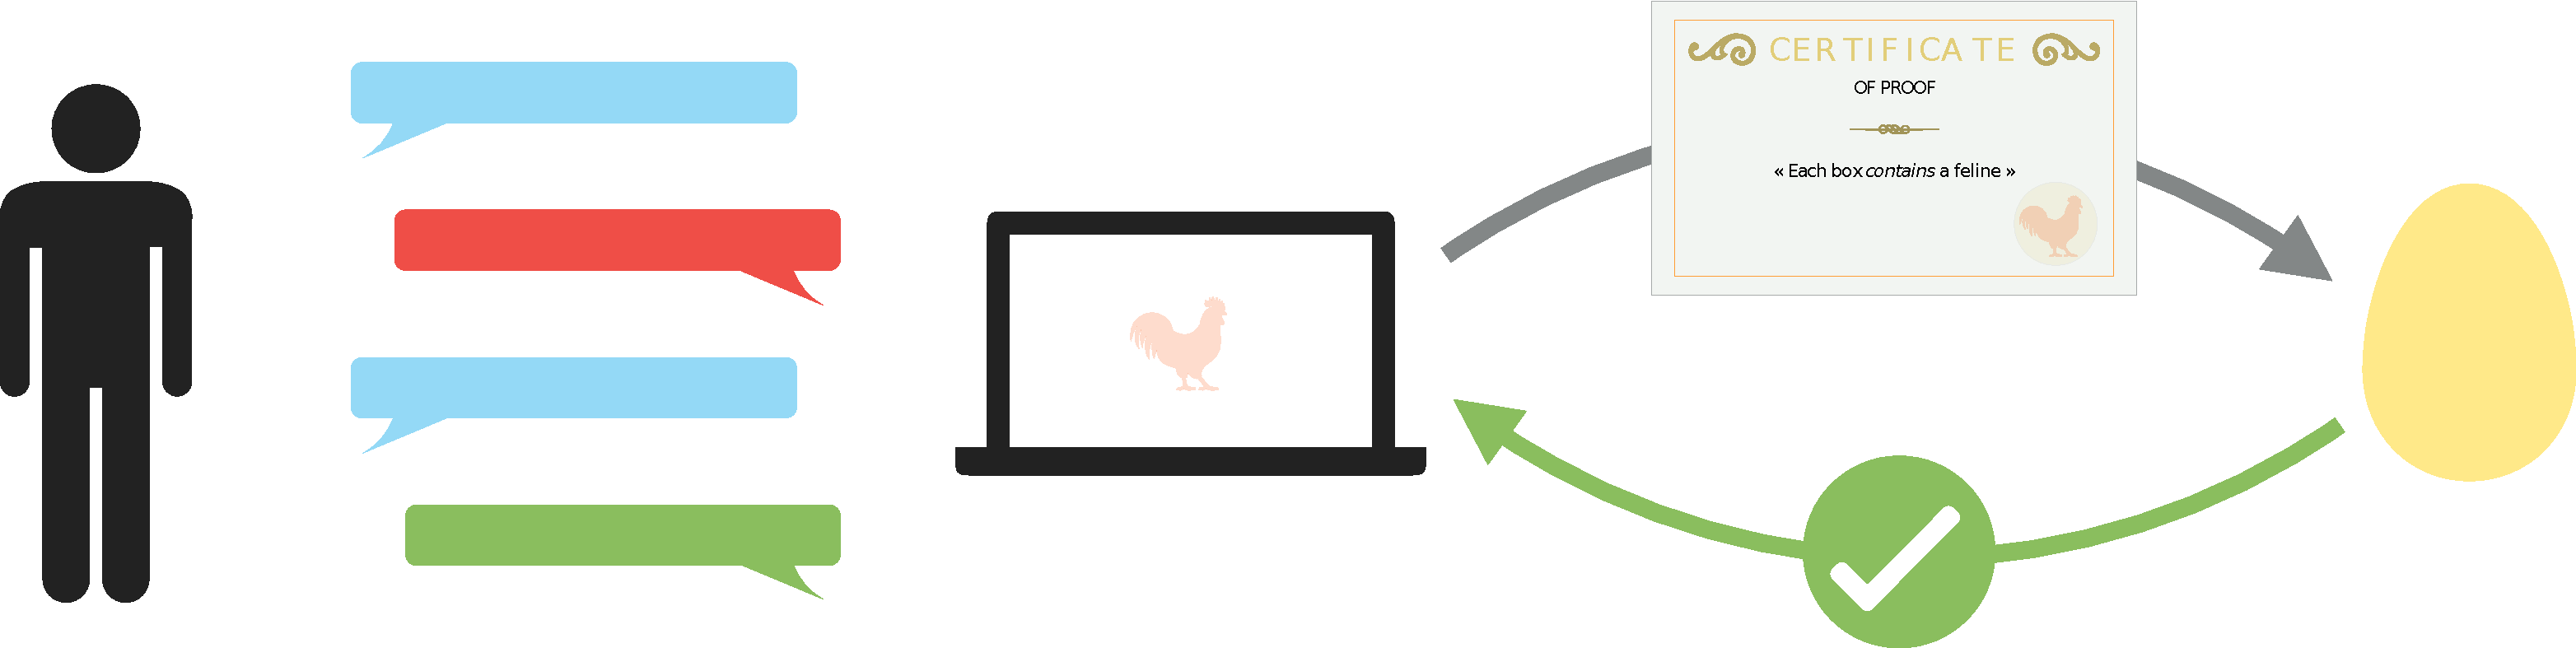
\includegraphics[width=0.9\textwidth]{chatbot-kernel.pdf}
\end{center}
\marginnote[-2.5cm]{
  The egg on the right represents the kernel. The proof assistant essentially
  sends it the certificate it generated after discussing with the user and the
  kernel validates it (or not).
}

If the proof assistant is broken, the certificate will be incorrect and rejected
by the kernel. As long as the kernel is correct, it is not crucial that the rest
is completly correct. Granted, it is nicer when everything is correct, but only
the correctness of the kernel is crucial.
As I said, efforts are made to keep the kernel as small as possible so that
humans can inspect it and assert of its correctness.

Unfortunately even a proof assistant as widely used as \Coq is not exempt from
mistakes: one critical bug had been found roughly every year for the past twenty
years. These are usually fixed rather quickly but their mere existence is
troublesome nonetheless.
An incorrect proof can have desastrous consequences. \Coq is not only used to
prove mathematical theorems, but also to verify programs and make sure they will
not crash or end up in unwanted configurations. Such programs that we want to
verify are often used in critical parts of softwares, for instance in autopilots
and rockets, where the smallest mistake can cost millions... and lives.

I am part of a project---the \MetaCoq project---to specificy and verify \Coq's
kernel itself, within \Coq. This means we produce a separate kernel, fully
written and verified in \Coq that can also check certificates independently.

When verifying the kernel we need to rely on meta-theoretical properties of
\Coq's theory. Unfortunately, not all of them can be proven within \Coq itself.
\marginnote[0.1cm]{
  I will talk about Gödel's incompleteness theorems in \nrefch{proof-theory}.
}%
This is because of Gödel's incompleteness theorems which roughly implies that a
theory like that of \Coq cannot prove its own consistency. As such, we need to
assume some of these meta-theoretical properties, especially those strong enough
to imply the consistency of \Coq, hence which cannot be proven.
Thus, we propose a paradigm shift: instead of having a relatively small kernel
that is trusted, we rely on a small base of properties assumed on the theory
which has been well studied over the years and does not suffer form the
shortcomings of the implementation.
There are other challenges we must face, one of which is proving that the
definitions we provide for the kernel are terminating, this was much more
complicated that anticipated and forced us to make explicit a lot of invariants
which are kept implicit (and sometimes unknown) in the current implementation.

All in all, we provide a specfication of \Coq, within \Coq, with a few trusted
properties about the theory with which we verify the soundness of an alternative
\Coq kernel.

\selectlanguage{english}